Dieses Kapitel beleuchtet dieser Arbeit zugrunde liegende Konzepte und Algorithmen. Zunächst wird das Prinzip der Epipolargeometrie beschrieben welches ein wesentlicher Bestandteil photogrammetrischer Verfahren ist. Daraufhin folgt eine Erläuterung des Terms Stereo Matching sowie eine Klassifizierung in lokale und globale Algorithmen. Im Anschluss daran wird das Prinzip des Block Matching Algorithmus grundlegend beschrieben, welcher die Grundlage für den im Rahmen dieser Arbeit verwendeten Semi Global Block Matching Algorithmus bildet. Anschließend erfolgt eine Erläuterung des verwendeten Frameworks sowie Details zur Implementierung dessen.

% ---------------------- section -----------------------
\section{Epipolargeometrie}
\label{sec:epipolargeometrie}
Bei der Verwendung der meisten photogrammetrischen Verfahren spielt die Epipolargeometrie eine entscheidende Rolle. Das mathematische Modell beschreibt die geometrische Beziehung zwischen verschiedenen Kamerabildern desselben Objektes, sowie die Beziehung korrespondierender Punkte. Generell gesehen ist die Epipolargeometrie durch das Lochkamera-Modell beschrieben. Dabei liegt jeder Punkt des aufgenommenen Objektes mit dem Projektionszentrum sowie dem Bildpunkt auf einer Geraden. Unter Zuhilfenahme der extrinsischen Orientierung sowie der intrinsischen Parameter der Kamera, ist es möglich den Schnittpunkt zweier Geraden zu berechnen um die dreidimensionalen Koordinaten des Objektpunktes zu erhalten. Dabei gilt generell, wenn ein Punkt $P$ im linken Bild gegeben ist, so wird die Suche des korrespondierenden Punktes $P’$ auf die Epipolarlinie des rechten Bildes reduziert. 

% GRAFIK: epipolargeometrie
\begin{figure}[h]
	\begin{center}
		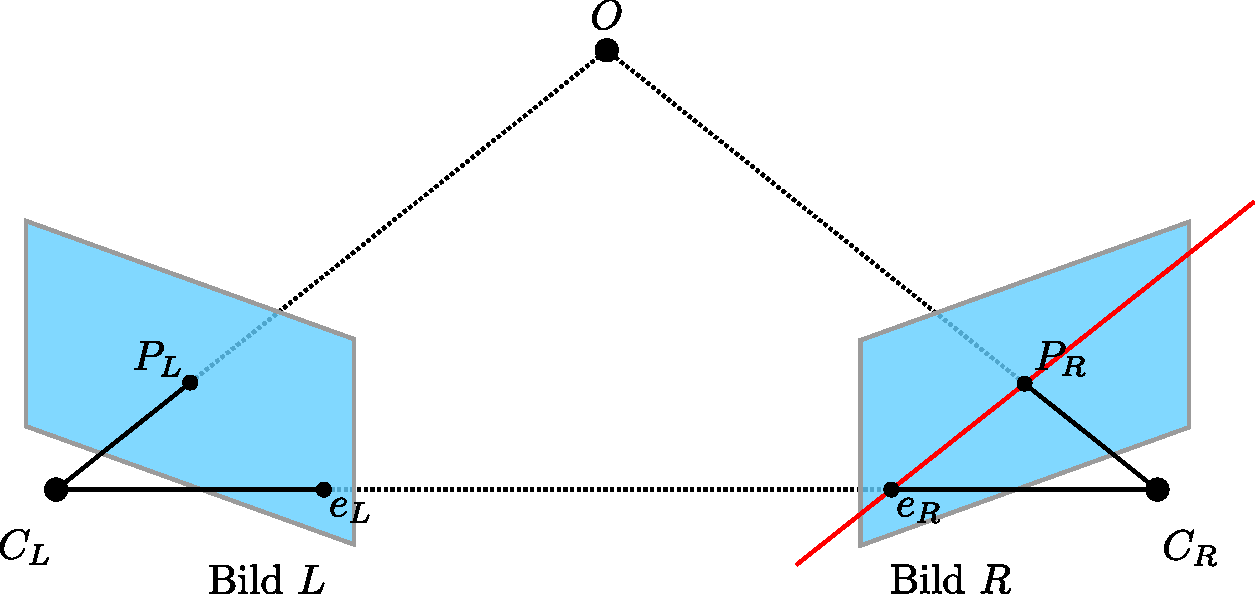
\includegraphics[width=10cm]{img/epipolar_geometry.pdf}
	\end{center}
	\caption{Darstellung der Epipolargeometrie.}
	\label{fig:epipolar_geometry}
\end{figure}

\noindent
Abbildung \ref{fig:epipolar_geometry} visualisiert diesen Prozess. Gegeben sind die beiden Projektionszentren $C_L$ und $C_R$ der beiden Bildebenen sowie die Bildpunkte $P_L$ und $P_R$. Der Objektpunkt $O$ bildet im linken Kamerabild auf $P_{x_1,y_1}$ ab. Zunächst ist es nur möglich den Strahl auf dem sich $O$ befindet zu bestimmen. Aufgrund des Wissens der extrinsischen Orientierung der Kameras können mithilfe der Basislinie zwischen den beiden Kameras die beiden Epipole in $L$ und $R$ ermittelt werden. Dabei sind diese durch den Schnittpunkt der Basislinie mit den beiden Bildebenen definiert \footnote{Im Falle eines Stereonormalfalles ist ein Schnittpunkt der Basislinie mit den Bildebenen nicht möglich, sodass die Epipole in der Unendlichkeit und parallel zur x-Achse liegen. Dies hat unter anderem den Vorteil, das die Epipolargeometrie bereits bekannt ist, und korrespondierende Bildpunkte nur noch innerhalb einer Pixelreihe gesucht werden müssen.}. Somit ist es möglich mithilfe der vorhandenen Epipole $e_L$, $e_R$ die Epipolarlinie $e_l,P_{x_2,y_2}$ zu bestimmten. Anhand dieser kann im Anschluss die dreidimensionale Position des Objektpunktes $O$ bestimmt werden.

\section{Kamerakalibrierung und Rektifizierung}
\label{sec:camera_calibration}
Um den Prozess des Stereo Matchings zu vereinfachen und beschleunigen bietet die Rektifizierung der Referenzbilder einen simplen Einstiegspunkt zur Lösung des Stereo-Korrespondenzproblems. Dafür müssen zunächst die intrinsischen und extrinsischen Parameter der Kamera berechnet werden. Dieser Prozess wird als Kalibierung der Kamera bezeichnet. Dafür werden Bilder eines Kalibierobjektes aufgenommen. Diese sind meistens einfache Schachbrettmuster mit ungleicher Anzahl an Quadraten, oder auch radiale Objekte mit einem spezifischerem Aufbau. Der Prozess der Kalibierung zielt darauf ab die \enquote{inneren} Parameter der Kamera zu bestimmen. Dies beinhaltet einerseits die Kameramatrix in welcher Parameter wie der Fokus Punkt(Focal Point), der Bildhauptpunkt(Principal Point) sowie die Brennweite der der Kamera. Weiterhin werden geometrische Verzerrungen des Bildes,  parametrisiert und somit nutzbar für die Entzerrung der Bilder in weiteren Schritten. Weiterhin werden bei der Kallibrierung die extrinsischen (äußeren) Parameter der Kamera bestimmt. Zu diesen zählt die Translation (x, y und z) sowie die Rotation der Kamera um die jeweiligen Achsen des Weltkoordinatensystems. Ein spezieller Aspekt bei der Kalibierung von Stereo-Systemen ist die Berechnung der extrinsischen Parameter von einer Kamera zur anderen. Die dabei berechnete Translation einer Kamera zur Referenzkamera wird als Baseline bezeichnet. Diese ist für Prozeduren wie Stereo-Matching unabdingbar. Der Prozess der Parameterfindung ist in der Regel ein Prozess welcher einmalig nach dem Aufbau ausgeführt werden muss und solange währt wie sich nichts am Aufbau der Kameras ändert (Objektive, Translation, Rotation).\\

\noindent
Folgend aus der Kalibrierung der Kameras beginnt der Prozess der Rektifizierung der Bilder. Dieser kann dabei in zwei Schritte unterteilt werden, einerseits die Berechung der Region of Interest, andererseits die Rektifizierung jedes aufgenommenen Einzelbildes. Mithilfe der zuvor berechneten intrinsischen und extrinsischen Parameter kann nun die Transformation der beiden Kamerabilder zueinander berechnet werden. Dies geschieht unter dem Aspekt der Epipolargeometrie. Nach der Rektifizierung und dem Anwenden der ROIs auf beiden Kamerabildern entspricht die jeweilige Pixelreihe im linken Bild der Pixelreihe mit dem selben Index im rechten Bild. Abbildung \ref{img:rectification} verdeutlicht den Ablauf der Rektifizierung, so ist in Abbildung \ref{img:rectification} (c) erkennbar das sich die korrespondierenden Bildpunkte auf einer Epipolarlinie befinden.\\
    % TODO retification beschreiben

   	\pagebreak
\begin{figure}[h]
	\centering
	\begin{tabular}{c}
	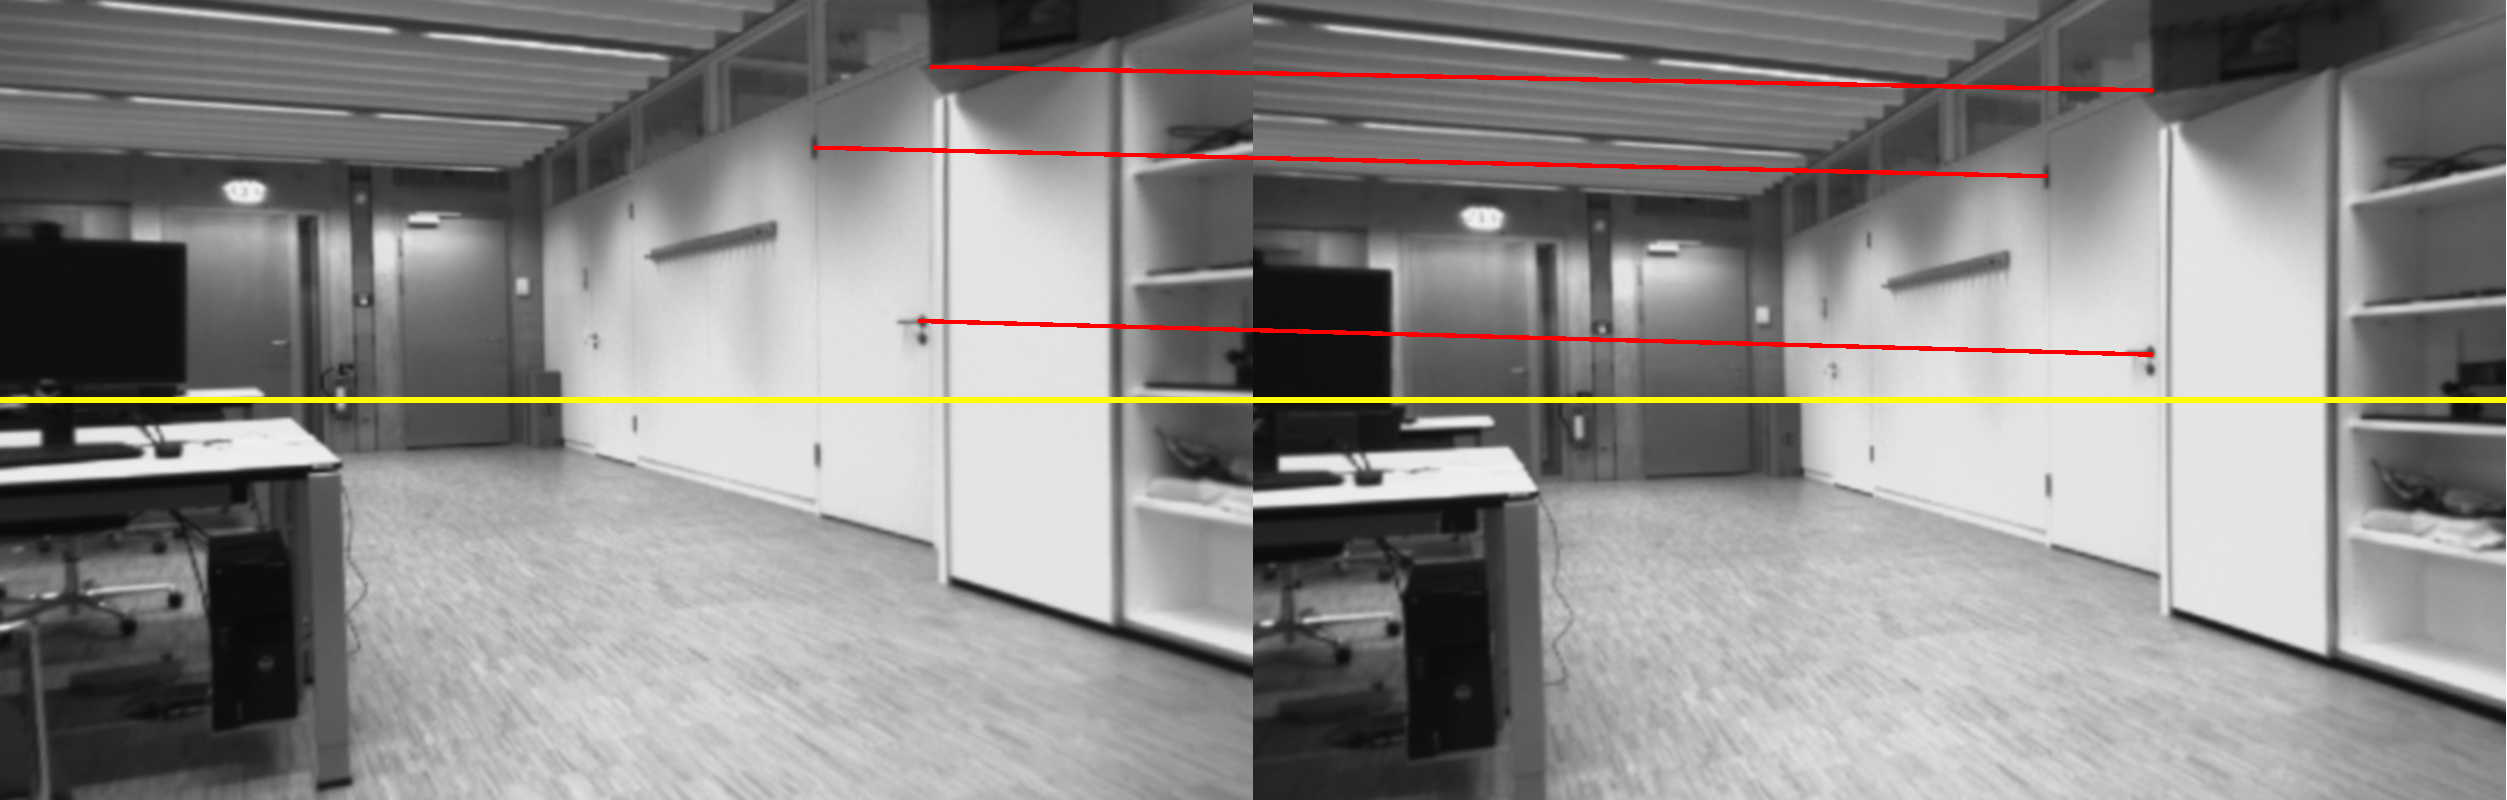
\includegraphics[width=10cm]{img/calibration/undistort}\\
	\small (a) Korrespondierende Punkte innerhalb der entzerrten Bilder\\\\
	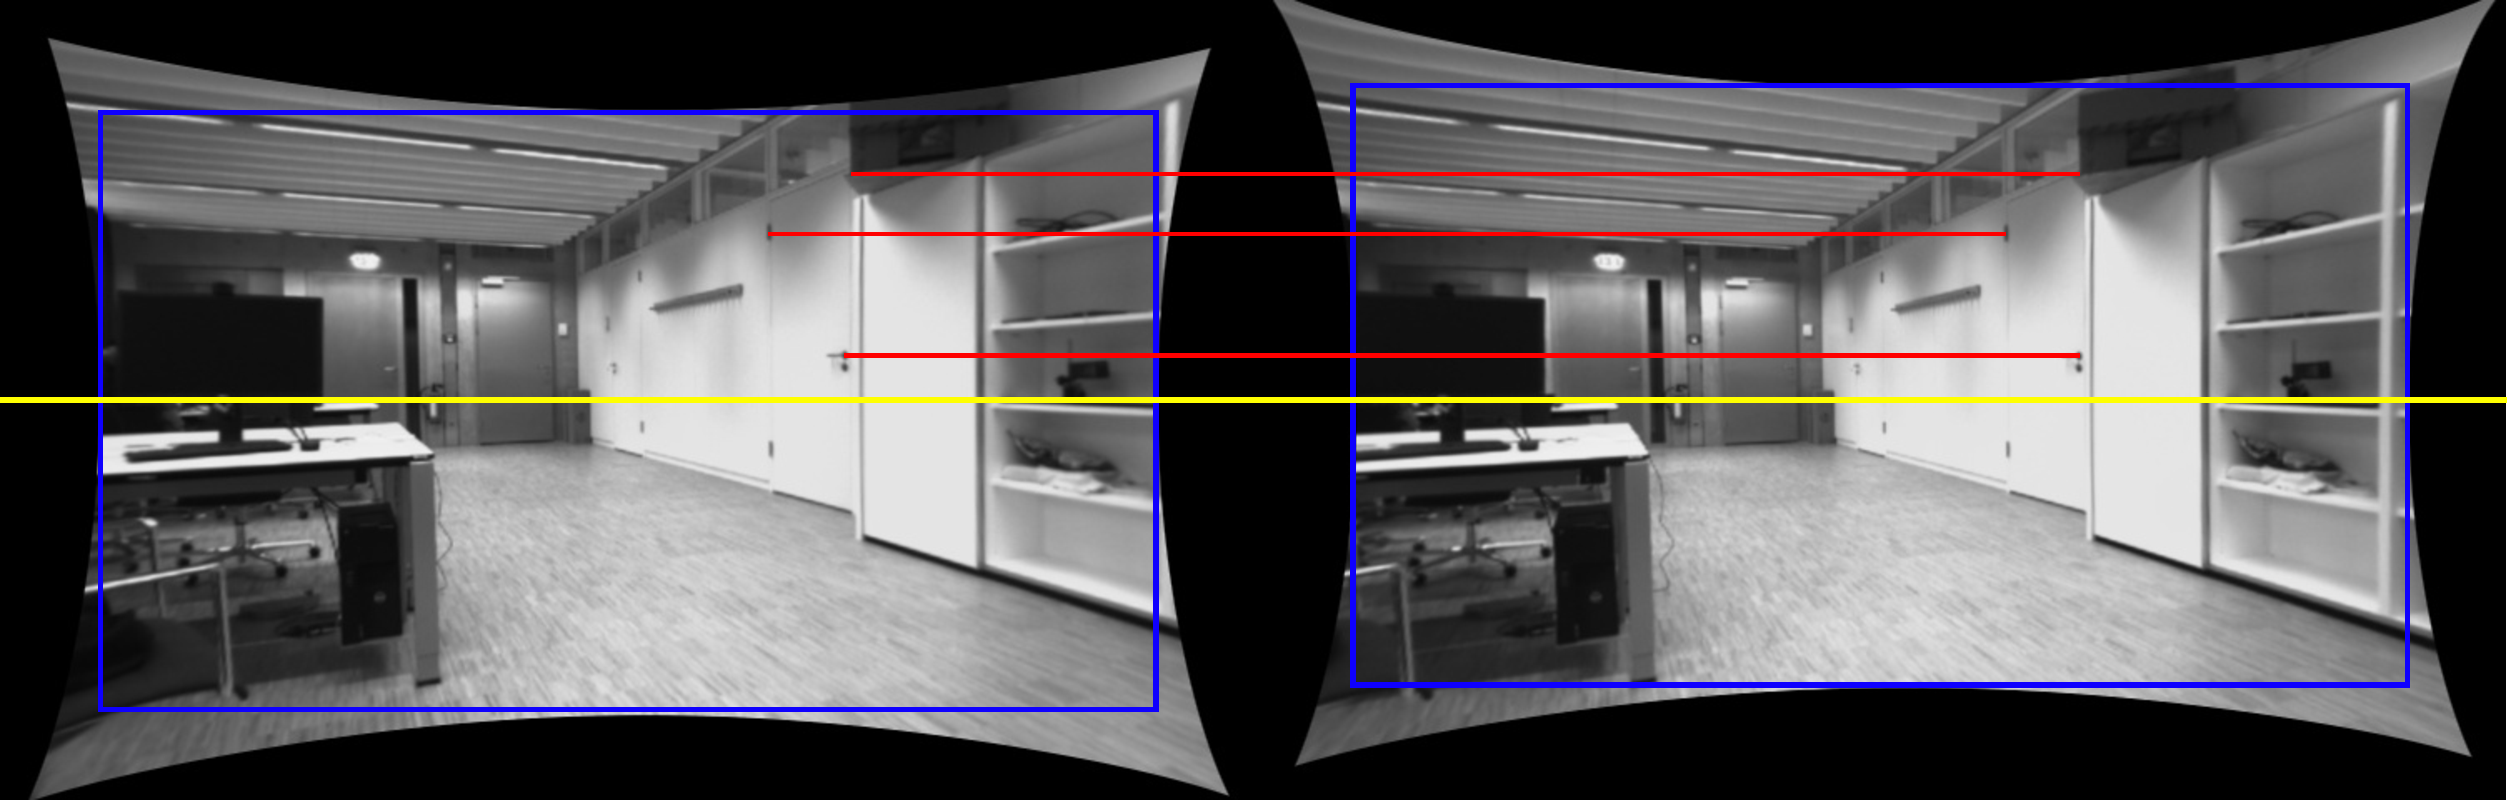
\includegraphics[width=10cm]{img/calibration/rect_uncropped.pdf}\\
	\small (b) Korrespondierende Punkte in den rektifizierten Bilder\\\\
	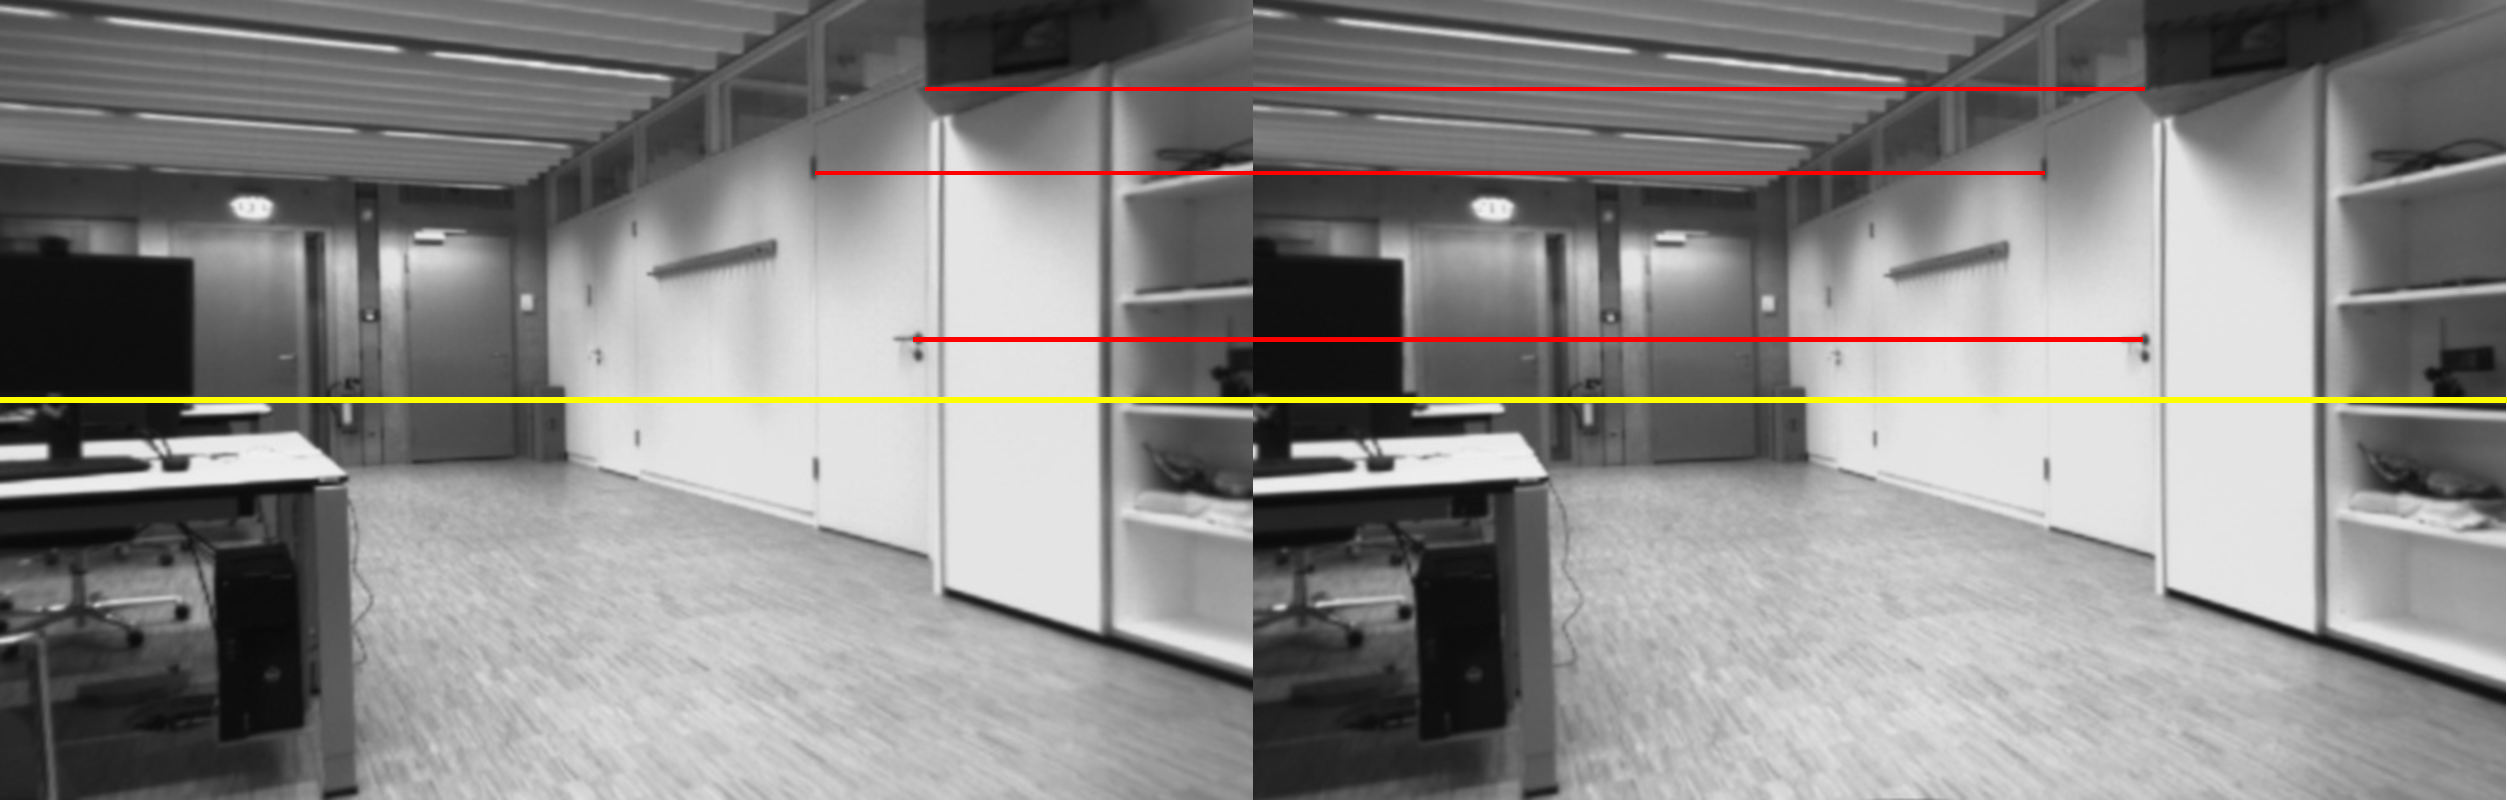
\includegraphics[width=10cm]{img/calibration/rect_cropped.pdf}\\
	\small (c) Korrespondierende Punkte in den geschnittenen und \\
				skalierten rektifizierten Bildern
	\end{tabular}
\caption{Resultat der Rektifizierung}
\label{img:rectification}
\end{figure}


% ---------------------- section -----------------------
\section{Stereo Matching}
\label{sec:stereo_matching}
Das grundlegende Konzept des Stereo Matchings beschreibt das Finden korrespondierender Punkte in zwei simultan aufgenommenen Bildern. Die Position der beiden Kameras ist dabei leicht versetzt, um einen jeweils anderen Blickwinkel auf die Szene zu erhalten. Mithilfe der verschiedenen Perspektiven können Disparitäten (Differenz der Projektion eines Objektes vom linken zum rechten Bild) zwischen korrespondierenden Pixeln berechnet werden. Die dabei erhaltenen Tiefeninformationen eines Objektes sind mit der errechneten Disparität sowie der relativen Position der Kameras und deren intrinsischen Parametern verbunden.
Im Laufe dieses Prozesses kommt es zu zwei wesentlichen Problemstellungen: die Berechnung der Disparität (Stereo Korrespondenz) sowie die Invertierung der projektiven Geometrie, um dreidimensionale Informationen aus der errechnetet Disparität zu erhalten. Sofern eine Lösung beider Probleme vorhanden ist, können diese Informationen durch einfache Triangulierung errechnet werden.

\subsection{Klassifikation}
\label{subsec:stereo_matching_classification}
\textbf{Lokale Methoden:}\\
Zur Berechnung der Disparität in lokalen Stereo Matching Algorithmen gilt grundlegendes Prinzip: “Finde Pixel $P_2$ korrespondierend zu $P_1$ im Referenzbild”. Dabei wird die Korrelation von $P_1$ und $P_2$ durch deren lokale Umgebung bestimmt. Der Referenzpunkt ist dabei das Zentrum eines Bereiches in welchem das Matching ausgeführt wird. Geläufige Methoden dafür sind Sum of Absolute Differences (SAD) (Hirschmüller 2011), Zero-mean Normalized Cross-Correlation (ZNCC) (Chen \& Medioni, 1999), (Sára, 2002), Sum of Squared Differences (SSD) (Cox et al., 1996), etc..
Jedoch können aufgrund fehlender Beschränkungen verzerrte Berechnungen der räumlichen Tiefe auftreten, da benachbarte Pixel verschiedene Disparitäten aufweisen können (beispielsweise an horizontalen Kanten wie Türrahmen etc.). Strukturell gesehen sind lokale Methoden einfacher gehalten als globale Methoden, wodurch ein hoher Grad an Optimierung in der Implementierung möglich ist.\\

\noindent
\textbf{Globale Methoden:}\\
Bei globalen Stereo Matching Algorithmen wird ein globales Modell der zu betrachtenden Szene erstellt sowie eine ebenfalls globale Kostenfunktion definiert, welche minimal gehalten werden soll. Dabei werden im Gegensatz zu lokalen Methoden die Matches in einer Pixelreihe und die des gesamten Bildes miteinander verglichen. Zusätzlich zu den benachbarten Pixeln werden hier ebenfalls die Matches der angrenzenden Pixel betrachtet. Zur Vereinfachung dieses Vorgangs betrachten einige Algorithmen nur die Epipolargeometrie, wobei ein zweidimensionales Problem auf ein eindimensionales reduziert wird. Resultierend daraus liegt die Stärke globaler Methoden in der Bewältigung schwacher Texturen sowie auftretender Okklusionen und unterschiedlicher Lichteinfälle, was, aufgrund der höheren Komplexität in einem höheren Rechen- und Speicheraufwand mündet. Weitere Verbesserungen der Ergebnisse können durch Techniken wie Dynamische Programmierung und Graph Cut erreicht werden.

\subsection{Block Matching}
\label{subsec:stereo_matching_bm}
Einen der einfachsten Ansätze zur Berechnung von Korrespondenz zwischen zwei Bildern bietet der Block Matching Algorithmus. Bei dieser lokalen Methode werden Blöcke bestimmter Größe mithilfe mathematischer Berechnungen (NCC, SAD, etc.) auf Korrespondenz untersucht. Dabei reduziert die Epipolargeometrie diesen Prozess auf ein eindimensionales Problem indem ein Block im linken Bild mit einem Block im rechten Bild auf der Epipolarlinie des rechten Bildes pixelweise vergleichen wird. Das eigentliche Matching erfolgt über die Berechnung eines Blockes mithilfe einer Energiefunktion.
% Dabei gilt es, bei der Korrespondenzanalyse mit dem möglichst gleichen Wert zu erhalten. 

%TODO: Block/Schrift groesser
\begin{figure}[h]
	\begin{center}
		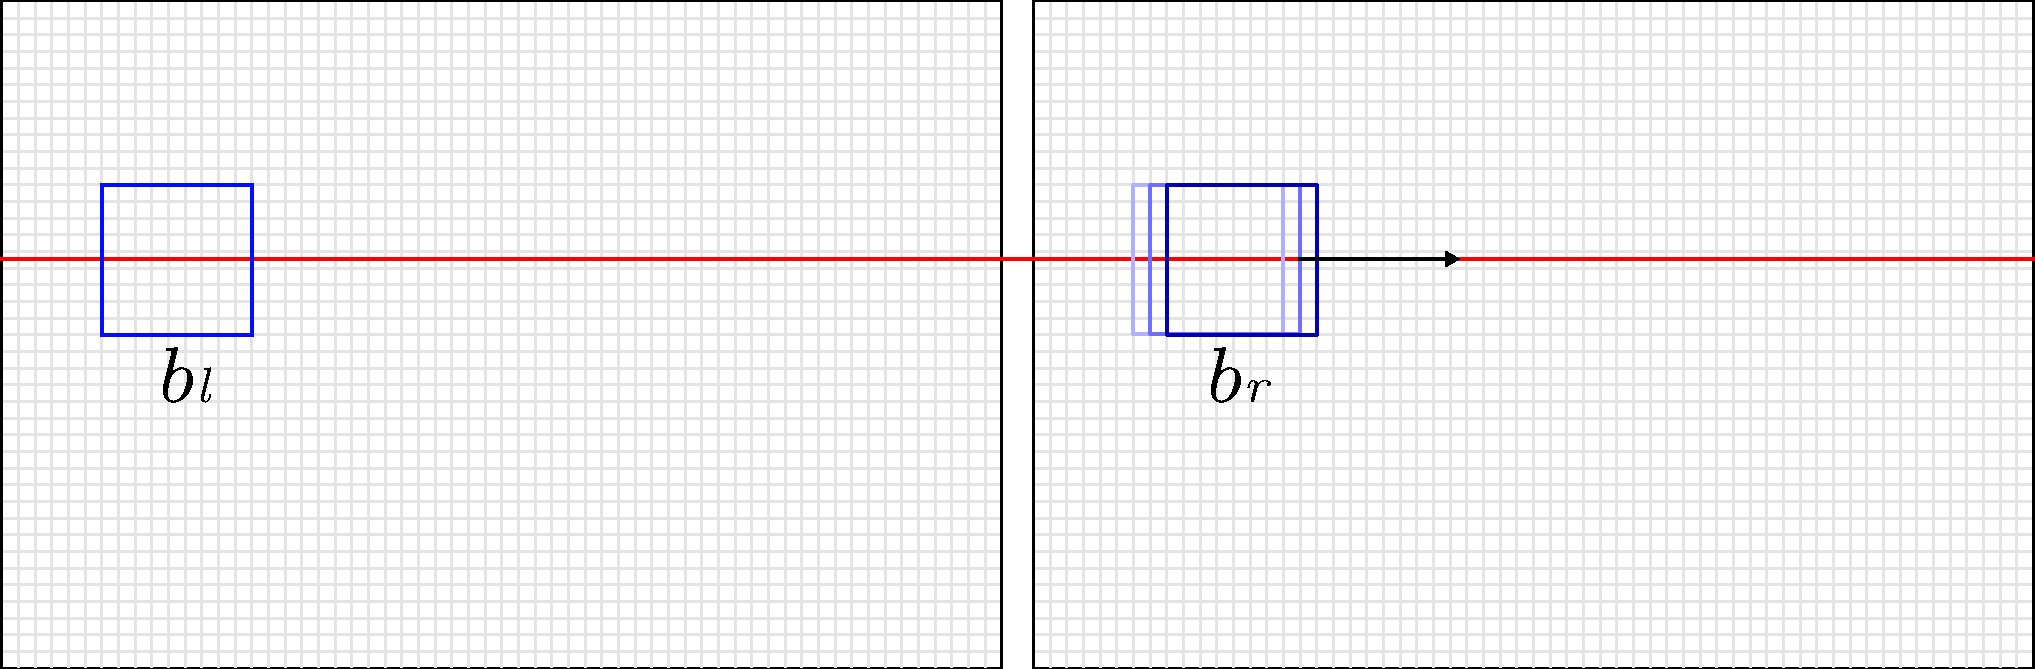
\includegraphics[width=10cm]{img/block_matching.pdf}
	\end{center}
	\caption{Visualisierung des Block Matching Algorithmus}
	\label{fig:block_matching}
\end{figure}

\noindent
Diesen Prozess veranschaulicht Abbildung \ref{fig:block_matching} . Durch den Fokus auf einzelne Pixelreihen und deren unmittelbare Umgebung ist dieses Verfahren wesentlich schneller, aber auch ungenauer als globale Matching Algorithmen. 
 

\subsection{Semi Global Block Matching}
\label{subsec:stereo_matching_sgbm}
Das im Rahmen dieser Arbeit verwendete Verfahren zur Berechnung von Disparity Maps ist der in der freien Computer Vision Library implementierte Semi Global Block Matching Algorithmus. Diese leicht abgewandelte Implementierung des Semi Global Matching Algorithmus von Hirschmüller et. al \cite{hirschmuller2005sgm} zeichnet sich sowohl durch seine Genauigkeit, als auch durch seine performante Berechnung aus. Unter Zuhilfenahme dieses Verfahren ist es möglich, Disparity Maps in Echtzeit mit sehr guter Framerate zu berechnen. Im Folgenden wird zunächst die grundlegende Funktionsweise des SGM erläutert. Im Anschluss daran werden die Unterschiede zum SGBM herausgearbeitet sowie eine kurze Erklärung der Parameter dessen vorgenommen.\\

%TODO: footnote Mutal Information fixen
\noindent
\textbf{SGM:} \\
Die grundlegende Idee des Semi-Global Matching Algorithmus besteht in dem pixelweisen Matching von Mutual Information \footnote{Mutual Information(MI), zu deutsch Transinformationen, beschreiben den statistischen Zusammenhang zweier Zufallsgrößen. Genauer gesagt beschreiben sie die Höhe des Informationsgehaltes einer Zufallsvariable aus anderen zufällig gewählten Werten.}. Die globale zweidimensionale Smoothness Einschränkung wird dabei mithilfe mehrerer eindimensionaler Einschränkungen erzeugt. Ausgangsvorraussetzung dafür sind verschiedene Bilder derselben Szene mit vorhandener und bekannter Epipolargeometrie. 
Zunächst werden für jeden Pixel $P$ aus der Intensität $I_{bp}$ sowie der vermuteten Korrespondenz $I_{mq}$ auf der Epipolarlinie $q=e_{bm}(pd)$ die Matching Kosten berechnet. Die eigentliche Berechnung dieser erfolgt dann mit Hilfe von Mutual Information berechnet.

\begin{equation}\label{eq:mutual_information_1}
MI_{I_1,I_2} = \sum_{p} mi_{I_1,I_2}(I_{1p},I_{2p})
\end{equation}
\begin{equation}\label{eq:mutual_information_2}
mi_{I_1,I_2} (i,k) = h_{I_1}(i)+h_{I_2}(k)-h_{I_1,I_2}(i,k)
\end{equation}

\noindent
Zur Berechnung der MI mithilfe der in \ref{eq:mutual_information_1} und \ref{eq:mutual_information_2} dargestellten Formeln wird zunächst eine Initial Disparity Map benötigt. Diese wird nach Kim et al’s \cite{zureiki2008stereo} Ansatz zufällig gewählt, um die Kosten berechnen zu können. Dies ist insbesondere für iterative Verfahren geeignet, da andernfalls die Berechnung verlangsamt werden könnte. Zur Steigerung der Performanz wird die Disparity Map zunähst nur auf halber Auflösung berechnet,  wodurch der Rechenaufwand um den Faktor $2 \cdot 3$ reduziert wird.Zur Vermeidung falscher Kostenberechnungen durch auftretende Noise innerhalb des Bildes nimmt der Algorithmus weitere Einschränkungen vor. Dabei werden die benachbarten Disparitäten in die Berechnung \ref{eq:disparity_calculation} mit einbezogen.

\begin{equation}\label{eq:disparity_calculation}
 foo = foo
\end{equation}

\noindent
Das letzte Problem besteht in der Berechnung der Korrespondenz sowie der daraus resultierenden Disparitäten. Dabei wird nach der Disparität $D$ mit der geringsten berechneten Energiefunktion gesucht. Anstatt nun einfach den minimalsten Pfad der Kosten zu summieren, werden alle Richtungen zur aktuellen Disparität mit einbezogen (siehe Abbildung \ref{fig:sgm_directions}).

\begin{figure}[h]
	\begin{center}
		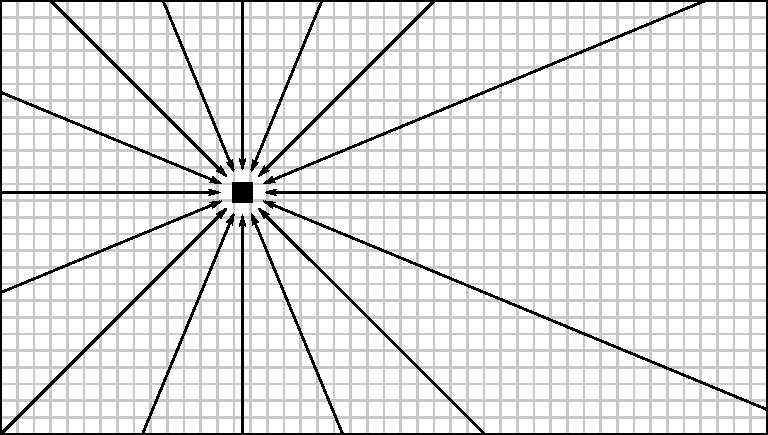
\includegraphics[width=8cm]{img/sgm_directions.pdf}
	\end{center}
	\caption{Darstellung der verschiedenen Richtungen}
	\label{fig:sgm_directions}
\end{figure}

\noindent
Zur Berechnung valider Werte sollten dabei mindestens 8 Richtungen vorliegen; -  eine vermehrte Anzahl an Richtungen, etwa 16, ist dabei vorteilhaft. Die berechnete Disparität ergibt sich aus den minimalen Kosten anhand dieser Pfade. Dabei gilt: “Je mehr Übereinstimmungen in den Kosten, desto wahrscheinlicher ist es, dass $D$ zur Intensität $I$ gehört”.\\

\noindent
\textbf{SGBM:} \\
Der Semi Global Block Matching Algorithmus ist ein in der Computer Vision Library OpenCV implementiertes Verfahren zur schnellen Berechnung von Disparity Maps. Die Grundlage dafür bietet Hirschmüller et al.’s SGM \cite{hirschmueller2008sgm} mit den folgenden grundlegenden Änderungen:

\begin{enumerate}[label=C.\arabic*]
	\item Statt den originalen 8 bzw. 16 Richtungen werden nur 5 betrachtet. \label{item:differences_directions}
	\item Es werden  standartm\"assig keine einzelnen Pixel sondern Blöcke verglichen. \label{item:differences_matching}
	\item Anstelle der Mutual Information Kostenfunktion wird das von Birchfield et al. vorgestellte Sub-Pixel Dissimilarity Measurement Verfahren verwendet \cite{birchfield-tomasi}.
	\item Pre und Post Processing Elemente des \emph{StereoBM} \cite{opencv_doc} werden verwendet.
\end{enumerate}

\noindent
%TODO: Parameter anpassung wichtig!, sgbm hirschmueller Mode!
Dies erlaubt dem Algorithmus eine schnelle Berechnung der Disparitäten auf einem qualitativ hochwertigen Niveau. Der geringe Verlust an Qualität kann in Anbetracht der Berechnung in Echtzeit vernachlässigt werden.

\begin{figure}[h]
\centering
	\begin{tabular}{m{2cm} m{3.3cm} m{3.3cm} m{3.3cm}}
	{\scriptsize Datensatz}&
	\begin{center} {\scriptsize Tskukuba} \end{center} &
	\begin{center} {\scriptsize Teddy} \end{center} &
	\begin{center} {\scriptsize Cones} \end{center}
	\\
	{\scriptsize Bilder links} &
	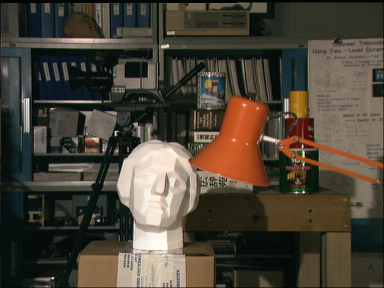
\includegraphics[width=3cm]{img/disparity_images/left_tsukuba.png} & 
	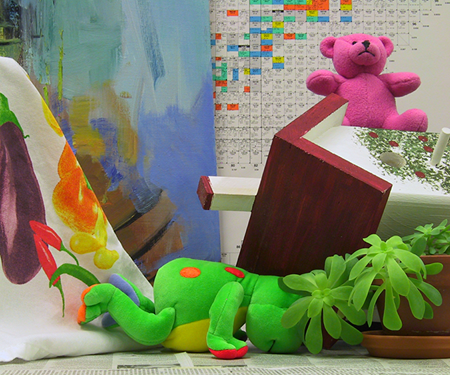
\includegraphics[width=3cm]{img/disparity_images/left_teddy.png} & 
	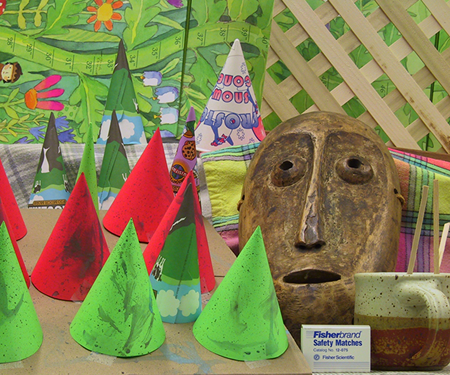
\includegraphics[width=3cm]{img/disparity_images/left_cones.png} 
	\\ 
	{\scriptsize Ground Truth} &
	
\includegraphics[width=3cm]{img/disparity_images/gt_tsukuba.png} & 
	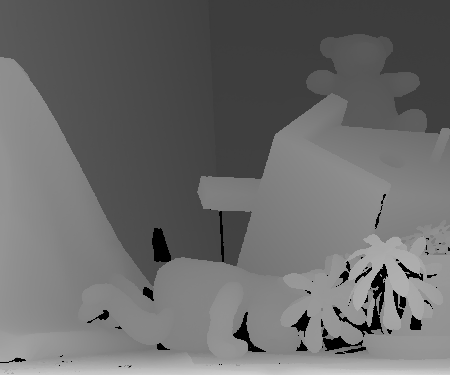
\includegraphics[width=3cm]{img/disparity_images/gt_teddy.png} & 
	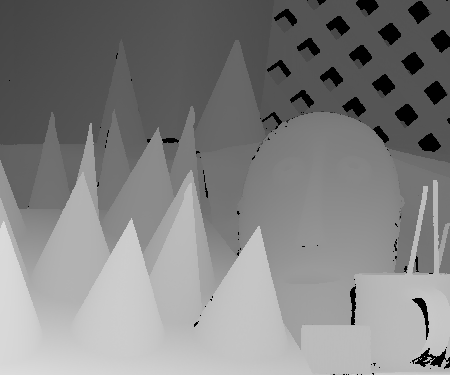
\includegraphics[width=3cm]{img/disparity_images/gt_cones.png} 
	\\
	{\scriptsize SGM (MI)} &
	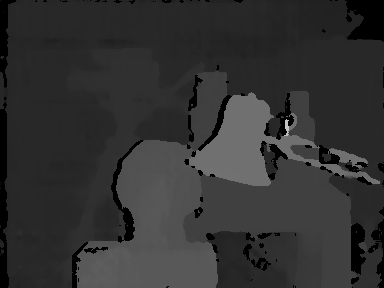
\includegraphics[width=3cm]{img/disparity_images/sgm_tsukuba.png} &
	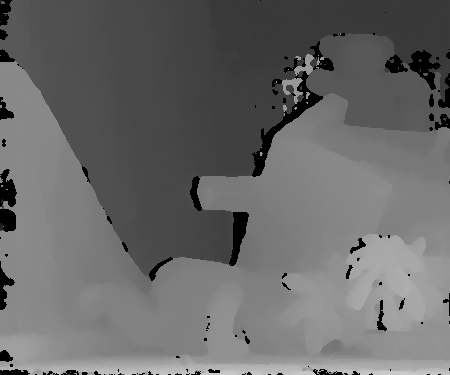
\includegraphics[width=3cm]{img/disparity_images/sgm_teddy.png} &
	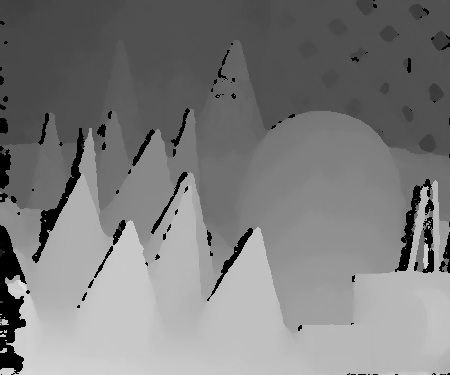
\includegraphics[width=3cm]{img/disparity_images/sgm_cones.png}
	\\ 
	{\scriptsize SGBM} &
	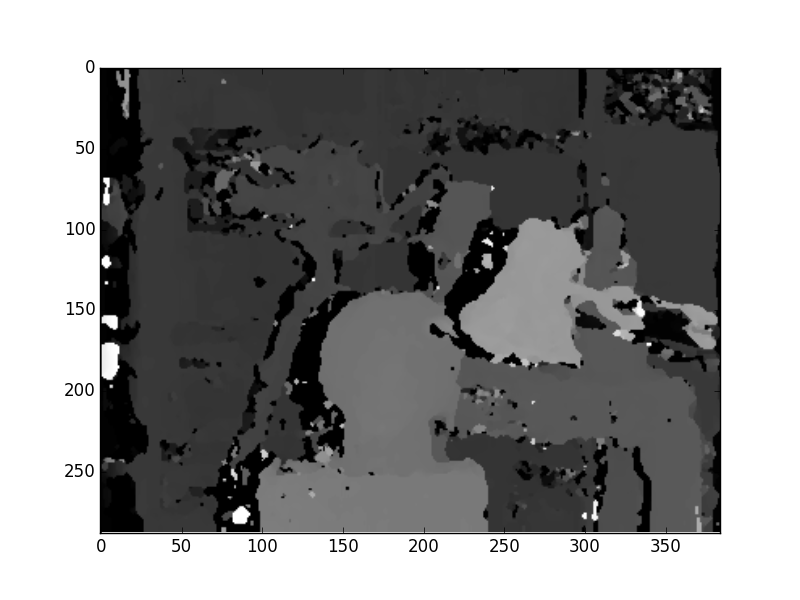
\includegraphics[width=3cm]{img/disparity_images/sgbm_tsukuba.png} &
	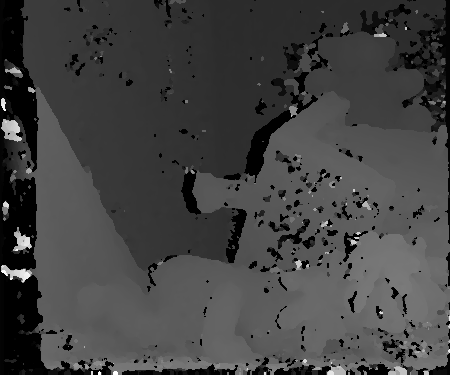
\includegraphics[width=3cm]{img/disparity_images/sgbm_teddy.png} &
	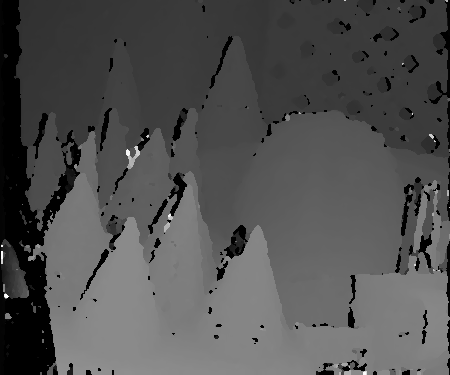
\includegraphics[width=3cm]{img/disparity_images/sgbm_cones.png}
	 \\ 
	\end{tabular}
\caption{Vergleich zwischen Ground Truth Bildern sowie dem SGM(2005) und OpenCV's SGBM}
\label{fig:disparity_comparison}
\end{figure}

\noindent
Abbildung \ref{fig:disparity_comparison} stellt die originalen Bildern der Szene (\cite{middlebury_data}), die mithilfe von strukturiertem Licht aufgenommenen Ground Truth Bilder sowie die jeweiligen berechneten Tiefenkarten durch den SGM und den SGBM dar. Aus dieser ist der Qualitaetsverlust des SGBM beim Tsukuba- sowie beim Teddy Datensatz zu erkennen. Trotz dessen sind die Grundformen sowie die berechnete Tiefe klar erkennbar. Grundlegend bietet der SGBM eine sowohl qualitativ hochwertige Berechnung von Tiefenkarten. Kleinere qualitative Einbußen können daher bei steigender Performanz akzeptiert werden.\\

\noindent
Weiterhin existiert eine Reihe verschiedener Parameter welche die Berechnung der Disparity Map aktiv beeinflussen. Im folgenden werden die zur Initialisierung obligatorischen Parameter in ihrer Funktionsweise grob beschrieben.

\begin{itemize}
	\item \textbf{\emph{minDisparity:}}\\
	Der Parameter \emph{minDisparity} begrenzt den messbaren Tiefenbereich nach oben, dies ist vor allem dann von Nöten wenn die Tiefenberechnung nach unten hin abgegrenzt werden soll. Er beschreibt also die minimale zu erkennende Disparität
 	\item \textbf{\emph{numDisparities:}}\\
 	Mit Hilfe der Number of Disparities \emph{numDisparities} wird die Breite des Matchingbereiches festgelegt. Er definiert wie viele Pixel im linken Bild auf Korrespondenz im rechten Bild analysiert werden sollen. In Abhängigkeit der Größe des Parameters entsteht bei der Berechnung der Tiefenkarte ein Bereich in welchem keine Informationen enthalten sind. Die damit verbundene weitere Verfahrensweise wird im Abschnitt \ref{sec:preprocessing} \enquote{Preprocessing} näher erläutert.
	\item \textbf{\emph{blockSize:}}\\
	Die \emph{blockSize} des \emph{SGBM} beschreibt die Größe des Matching Blocks in Pixeln. Je größer der Wert gewählt wird, desto weicher wird die resultierende Disparity Map. Dabei gehen jedoch auch Informationen verloren. Ist der Wert niedrig so ist es unter Umständen schwerer homogene Flächen korrekt zu Matchen und es treten mehr nicht-korrespondierende Bereiche auf.
\end{itemize}

% ---------------------- section -----------------------
\section{mvStereoVision Framework}
\label{sec:framework}
Das verwendete Framework zur Bildaufnahme und Disparity Map Berechnung wurde im Rahmen des Projektes “SLAM for UAV” entwickelt. Dieses bedient sich der von Matrix Vision zur Verfügung gestellte Library \cite{matrixvision} zur Kommunikation mit den Kameras, sowie OpenCV \cite{opencv} zur Verarbeitung der Bilder. Die wesentlichen Funktionen werden im folgenden näher beleuchtet.\\

\noindent
\textbf{Bildaufnahme:}\\
Die Aufnahme der einzelnen Bilder beginnt bei einer Anfrage an die Kamera nach den jeweiligen Rohdaten. Diese werden anschliessend mithilfe der durch die Kalibrierung ermittelten Parameter entzerrt und rektifiziert und liegen so zur weiteren Verarbeitung bereit. Die Aufnahme der Bilder erfolgt dabei in separaten Threads um unabhängig von weiteren Berechnungen Bilder aufzunehmen. Die Berechnung der Disparity Map erfolg ebenfalls in einem eigenen Thread. Sofern eine neue Disparity Map vorliegt wird innerhalb des Hauptprogramms mit Hilfe eines Wahrheitswertes darüber informiert das diese vorliegt. Der gesamte Prozess wird in Abbildung \ref{fig:framework_pipeline} visualisiert.\\

\begin{figure}[h]
	% TODO add another state for further processing
	\begin{center}
		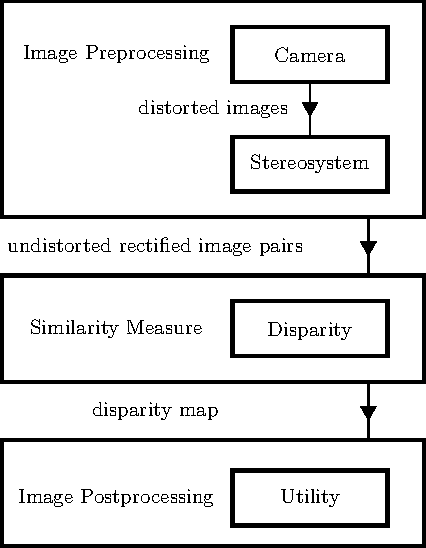
\includegraphics[width=6cm]{img/framework_pipeline.pdf}
	\end{center}
	\caption{Pipeline zur Bildaufnahme, Disparity Map Berechnung sowie weiteren Verarbeitung}
	\label{fig:framework_pipeline}
\end{figure}


\noindent
\textbf{Distanzberechnung:}\\
Zugrundeliegend bei der Distanzberechnung ist die Reprojektionsmatrix $Q$ welche im Rahmen der Rektifizierung berechnet wird und wie folgt aufgebaut ist.
\begin{equation}
    Q= 
    \begin{bmatrix}
      1 & 0 & 0 & -C_x\\
      0 & 1 & 0 & -C_y\\
      0 & 0 & 0 & f\\
      0 & 0 & \frac{-1}{T_x} & \frac{C_x - C_x'}{T_x}
    \end{bmatrix}
    \longrightarrow
    \begin{bmatrix}
      1 & 0 & 0 & -C_x\\
      0 & 1 & 0 & -C_y\\
      0 & 0 & 0 & f\\
      0 & 0 & a & b
    \end{bmatrix}
\end{equation}
Dabei beschreiben $-C_x$ und $-C_y$ die beiden negativen Koordinaten des Bildhauptpunktes der linken Kamera sofern dies als Referenz vorlag, der Parameter $f$ die Brennweite der linken Kamera. $T_x$ ist die horizontale Translation zwischen beiden Kameras. Die in der Q-Matrix enthaltenen Parameter sind mit Ausnahme von $C_x'$ alle die der linken Kamera. Es wird angenommen das sich die beiden Strahlen der Bildhauptpunkte in der Unendlichkeit schneiden woraus sich der Parameter $0$ in der unteren rechten Ecke berechnet. Zur Einfacheren Darstellung und Erläuterung werden die Baseline der Kamera $\frac{-1}{T_x}$ im folgenden als $a$ sowie die Darstellung beider Bildhauptpunkte $\frac{C_x - C_x'}{T_x}$ als $b$ notiert.\\

\noindent
Eine Eigenschaft der Reprojektionsmatrix ist die einfache Berechnung von dreidimensionalen Weltkoordinaten. Diese Berechnung ist in Formel \ref{eq:distance_calculation} abgebildet.

\begin{equation}\label{eq:distance_calculation}
    \begin{aligned}
        \begin{bmatrix}
            X\\ Y \\ Z\\ W
        \end{bmatrix}
        = Q \cdot 
        \begin{bmatrix}
            I_x\\ I_y \\ d(x,y)\\ 1
        \end{bmatrix}\\
        pointcloud(x,y) = [\frac{X}{W}, \frac{Y}{W}, \frac{Z}{W} ]
    \end{aligned}
\end{equation}

\noindent
Die eigentliche Berechnung der einzelnen Parameter ergibt sich somit aus der Multiplikation des transponierten Vektors, welcher sowohl die Koordinaten des Pixels als auch die Disparität dessen enthält, und der Reprojektions Matrix. Die dabei benötigten Operationen werden im folgenden genauer beleuchtet.


\begin{equation}
  \begin{aligned}
        X &= I_x - C_x\\
        Y &= I_y - C_y\\
        Z &= f\\
        W &= d \cdot a + b
  \end{aligned}
\end{equation}